\newpage
\refstepcounter{section}
%Add Image
\vspace*{-40mm} %Make image have no top margin
\begin{tikzpicture}
\node[inner sep=0pt] (x) at (0,0)
    {\hspace{-87mm}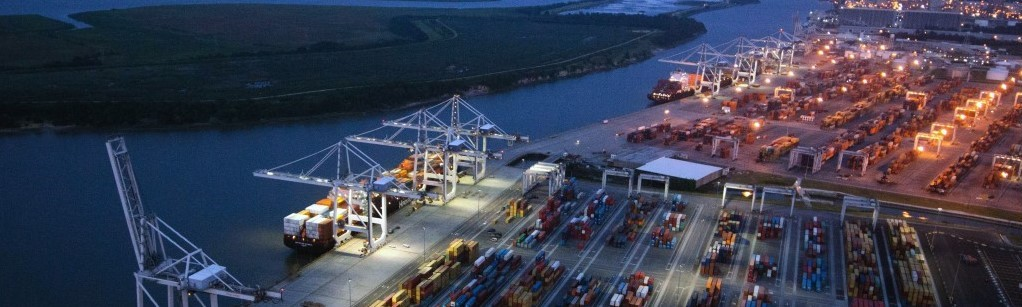
\includegraphics[width=\paperwidth]{sectionimage2.jpg}};
\node[text width=10in] (Z) at (0,-1) {\color{white}\headingfont\Large\bfseries\uppercase{\hspace{-0.7cm}\thesection\hspace{0.5cm}Risks}};
\end{tikzpicture}
%Modify TOC
\addcontentsline{toc}{section}{\protect\numberline{\thesection}Risks}
  \sectionmark{Risks}
\vspace{-2mm}

%Content

\begin{wraptable}{l}{\linewidth}
\centering
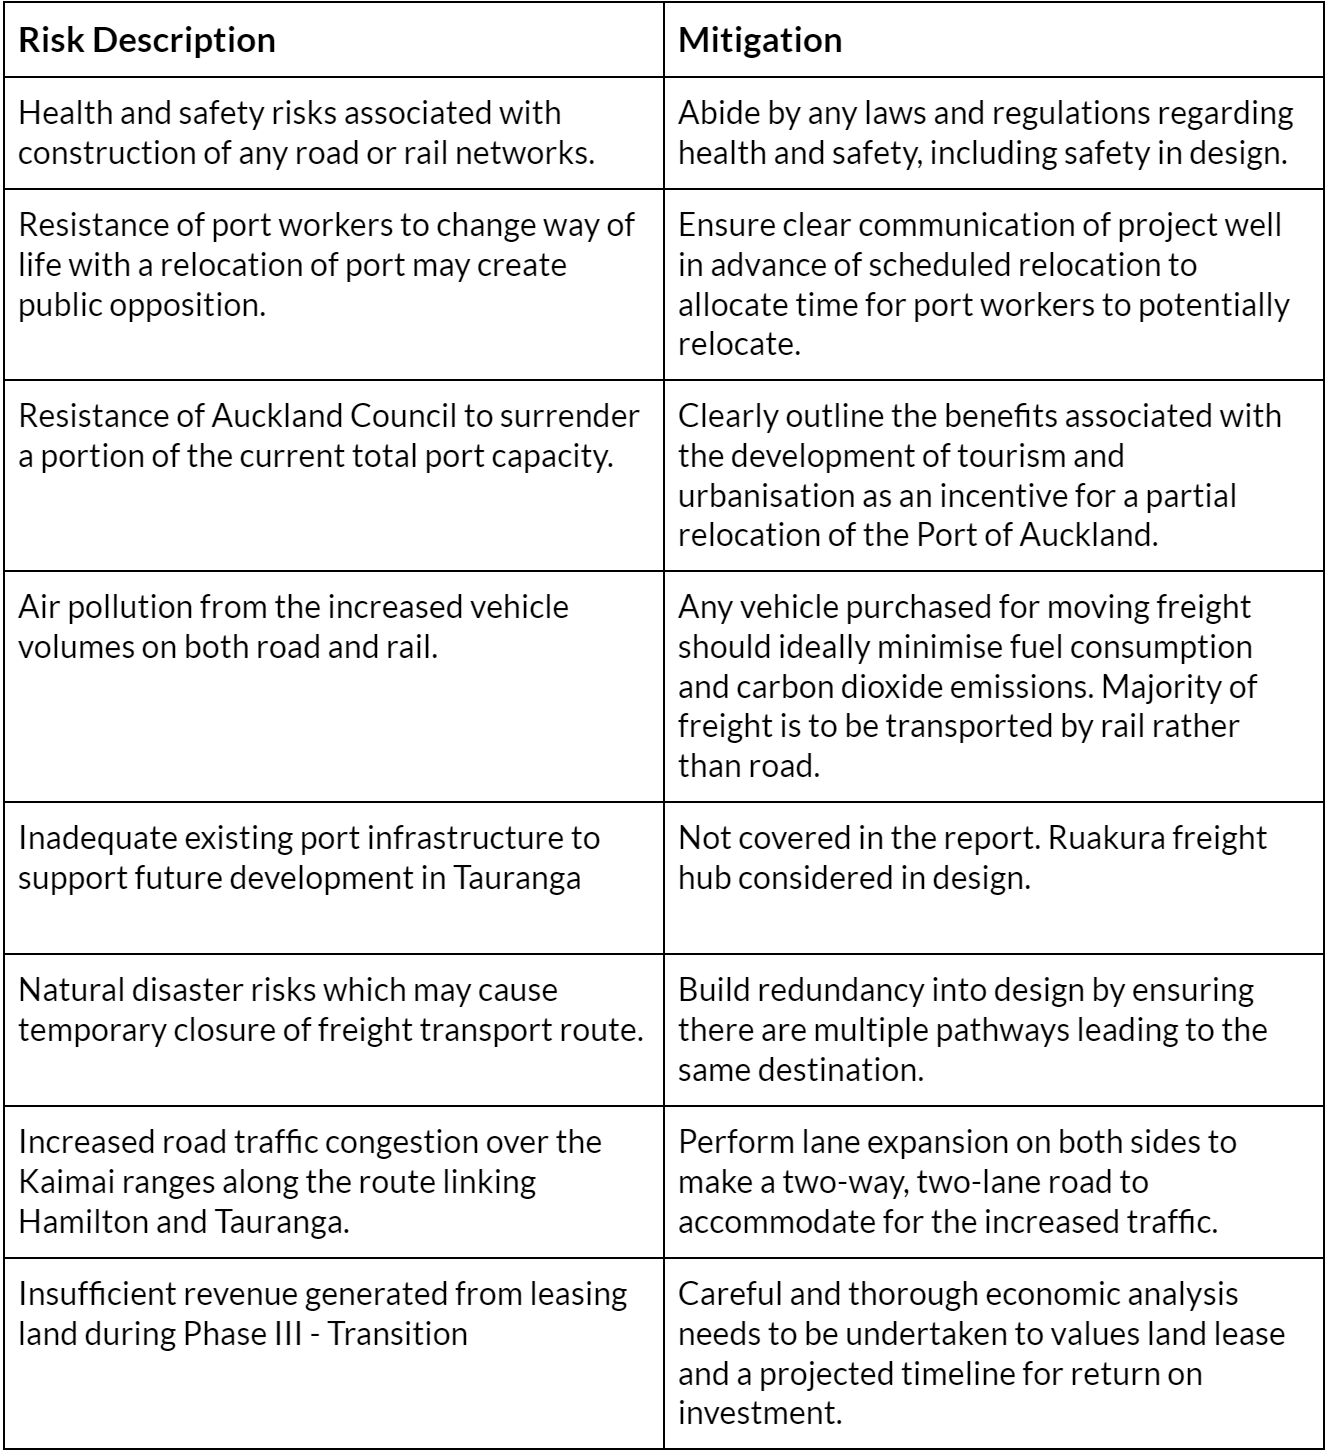
\includegraphics[width=\textwidth]{risks.png}
\centering
\caption{Table of Potential Risks}
\end{wraptable}


% \begin{multicols}{2}
% \subsection*{Health and Safety Risks Associated with Construction of any Road or Rail Networks}
%     \textbf{Mitigation: }{Abide by any laws and regulations regarding health and safety, including safety in design.}

% \subsection*{Resistance of port workers to change way of life with a relocation of port may create public opposition}
%     \textbf{Mitigation: }{Ensure clear communication of project well in advance of scheduled relocation to allocate time for port workers to potentially relocate.}

% \subsection*{Resistance of Auckland Council to surrender a portion of the port capacity}
%     \textbf{Mitigation: }{Clearly outline the benefits associated with the development of tourism and urbanisation as an incentive for a partial relocation of the Port of Auckland.}

% \subsection*{Air pollution from the increased vehicle volumes on both road and rail}
%     \textbf{Mitigation: }{Any vehicle purchased for moving freight should ideally minimise fuel consumption and carbon dioxide emissions. Majority of freight is to be transported by rail rather than road.}
    
% \subsection*{Inadequate existing port infrastructure to support future development in Tauranga}
%     \textbf{Mitigation: }{Not covered in the report. Ruakura freight hub considered in design.}    
    
% \subsection*{Natural disaster risks which may cause temporary closure of freight transport route}
%     \textbf{Mitigation: }{Build redundancy into design by ensuring there are multiple pathways leading to the same destination.}

% \subsection*{Increased road traffic congestion over the         Kaimai ranges along the route linking Hamilton and          Tauranga}
%     \textbf{Mitigation: }{Perform lane expansion on both sides to make a two-way, two-lane road to accommodate for the increased traffic.}
   
% \subsection*{Insufficient revenue generated from leasing land during Phase III - Transition}
%     \textbf{Mitigation: }{Careful and thorough economic analysis needs to be undertaken to values land lease and a projected timeline for return on investment.}   
   
% \end{multicols} 


\clearpage